% ------------------------------------------------------------------------
% ------------------------------------------------------------------------
% Modelo de relatório da equipe CEFAST AeroDesign
% ------------------------------------------------------------------------
% Modelo Baseado no código fornecido pela equipe do ITA,
% Disponível em: https://aerodesignita.wordpress.com/2015/07/19/modelo-de-relatorio-aerodesign-em-latex/
%
% Usamos e abusamos de:
% abnTeX2: Modelo de Relatório Técnico/Acadêmico em conformidade com 
% ABNT NBR 10719:2011 Informação e documentação - Relatório técnico e/ou
% científico - Apresentação
%
% ------------------------------------------------------------------------ 
% ------------------------------------------------------------------------

%Parte de formatação
\documentclass[
	% -- opções da classe memoir --
	12pt,				% tamanho da fonte
	oneside,			% para impressão em verso e anverso. Oposto a oneside
	a4paper,			% tamanho do papel. 
	% -- opções da classe abntex2 --
	%chapter=TITLE,		% títulos de capítulos convertidos em letras maiúsculas
	%section=TITLE,		% títulos de seções convertidos em letras maiúsculas
	%subsection=TITLE,	% títulos de subseções convertidos em letras maiúsculas
	%subsubsection=TITLE,% títulos de subsubseções convertidos em letras maiúsculas
	% -- opções do pacote babel --
	english,			% idioma adicional para hifenização
	spanish,			% idioma adicional para hifenização
	brazil,				% o último idioma é o principal do documento
	]{AeroDesign} 		% Estilo .cls pro AeroDesign (capa bodosa)


% ---
% PACOTES
% ---

% ---
% Pacotes fundamentais 
% ---
\usepackage{float}
\usepackage{lmodern}			% Usa a fonte Latin Modern
\usepackage[T1]{fontenc}		% Selecao de codigos de fonte.
\usepackage[utf8]{inputenc}		% Codificacao do documento (conversão automática dos acentos)
\usepackage{indentfirst}		% Indenta o primeiro parágrafo de cada seção.
\usepackage{color}				% Controle das cores
\usepackage{graphicx}			% Inclusão de gráficos
\usepackage{microtype} 			% para melhorias de justificação
\usepackage{pstricks}
\graphicspath{{IMG/}}
%##############
\usepackage{tabu}				% usar ambiente tabu no lugar de tabular
\setlength{\tabulinesep}{1.2mm} % Espaçando itens nas celulas da tabela
%##############

% ---
% Pacotes de citações
% ---
\usepackage[brazilian,hyperpageref]{backref}	 % Paginas com as citações na bibl
\usepackage[alf]{abntex2cite}	% Citações padrão ABNT

% --- 
% CONFIGURAÇÕES DE PACOTES
% --- 

% ---
% Configurações do pacote backref
% Usado sem a opção hyperpageref de backref
\renewcommand{\backrefpagesname}{Citado na(s) página(s):~}
% Texto padrão antes do número das páginas
\renewcommand{\backref}{}
% Define os textos da citação
\renewcommand*{\backrefalt}[4]{
	\ifcase #1 %
		Nenhuma citação no texto.%
	\or
		Citado na página #2.%
	\else
		Citado #1 vezes nas páginas #2.%
	\fi}%

% -------------------------------------------
% Informações de dados para CAPA e FOLHA DE ROSTO
% Informar o numero da equipe 
% O título é o nome da equipe!
% Colocar todos os membros como autores, pode colocar \at email se quiser..
% ---
\renewcommand{\nrEquipe}{06}
\titulo{Relatório Técnico de Elétrica}
\autor{
	Antônio Sousa \\
	Gabriel Viana \\
	Gustavo Pereira \\
	Leonardo Vaz \\
	Renato Freitas \\
	Tiago Dornelas \\
	\textbf{Piloto} - Rodrigo Zanasi
}
\local{Brasil}
\data{2017, v-1.0}
\instituicao{CENTRO FEDERAL DE EDUCAÇÃO TECNOLÓGICA DE MINAS GERAIS}
\orientador{Anthony Chiaratti}
\tipotrabalho{Relatório técnico}

% Configurações de aparência do PDF final

% alterando o aspecto da cor azul
\definecolor{blue}{RGB}{41,5,195}

% ---
% Identificando a categoria da equipe pela numeração
% ---

\global\edef\nrEquipepx{\nrEquipe,px}
\ifdim \nrEquipepx>200px
\definecolor{bgEquipe}{RGB}{0,190,100}
\renewcommand{\clEquipe}{Classe Micro}
\else
\definecolor{bgEquipe}{RGB}{0,128,255}
\renewcommand{\clEquipe}{Classe Advanced}
\fi
\ifdim \nrEquipepx<100px
\definecolor{bgEquipe}{RGB}{255,60,0}
\renewcommand{\clEquipe}{Classe Regular}
\fi
% informações do PDF
\makeatletter
\hypersetup{
     	%pagebackref=true,
		pdftitle={\@title}, 
		pdfauthor={\@author},
    	pdfsubject={\imprimirpreambulo},
	    pdfcreator={LaTeX with abnTeX2},
		pdfkeywords={AeroDesign}{SAE Brasil}{abntex}{abntex2}{relatório técnico}, 
		colorlinks=true,       		% false: boxed links; true: colored links
    	linkcolor=red,          	% color of internal links
    	citecolor=blue,        		% color of links to bibliography
    	filecolor=magenta,      		% color of file links
		urlcolor=blue,
		bookmarksdepth=4
}
\makeatother

% --- 
% Espaçamentos entre linhas e parágrafos 
% --- 

% O tamanho do parágrafo é dado por:
\setlength{\parindent}{1.3cm}

% Controle do espaçamento entre um parágrafo e outro:
\setlength{\parskip}{0.2cm}  % tente também \onelineskip

% Espaçamento de itens dentro da celula
\setlength{\tabulinesep}{1.2mm}
% ---
% compila o indice
% ---
\makeindex
% ---

% ----
% Início do documento
% ----
\begin{document}

% Seleciona o idioma do documento (conforme pacotes do babel)
%\selectlanguage{english}
\selectlanguage{brazil}

% Retira espaço extra obsoleto entre as frases.
\frenchspacing 

% ----------------------------------------------------------
% ELEMENTOS PRÉ-TEXTUAIS
% ----------------------------------------------------------
% \pretextual

% ---
% Capa
% ---
\imprimircapa
% ---

% ---
% Agradecimentos
% ---
\begin{agradecimentos}

Agradecemos aos voluntários que desenvolveram o pacote Abntex 2!
\end{agradecimentos}

% ---
% inserir lista de símbolos
% ---
\begin{simbolos}

\item[$\alpha$] Ângulo de ataque
\item[$\alpha _s$] Ângulo de ataque de estol
\item[$\beta$] Ângulo de derrapagem
\item[$\varphi$] Ângulo de inclinação lateral
\item[$\theta$] Ângulo de atitude
\item[$\psi$] Ângulo de proa
\item[$C_{m_{\alpha}}$] Derivada do coeficiente de momento de arfagem com relação ao ângulo de ataque
\item[$C_{L_{\alpha}}$] Derivada do coeficiente de sustentação com relação ao ângulo de ataque
\item[$C_{l_{\beta}}$] Derivada do coeficiente de momento de rolamento com relação ao ângulo de derrapagem
\item[$C_{n_{\beta}}$] Derivada do coeficiente de momento de guinada com relação ao ângulo de derrapagem
\item[$\delta _a$] Deflexão de aileron
\item[$\delta _p$] Deflexão de profundor
\item[$\delta _l$] Deflexão de leme
\item[$\delta _m$] Comando de manete
\item[$C_L$] Coeficiente de sustentação
\item[$C_M$] Coeficiente de momento de arfagem
\item[$C_{HT}$] Coeficiente de volume de cauda horizontal
\item[$C_{VT}$] Coeficiente de volume de cauda vertical
\item[$c_l$] Coeficiente de sustentação de perfil
\item[$V$] Velocidade
\item[$V_{stall}$] Velocidade de estol
\item[$V_{man}$] Velocidade de manobra
\item[$V_{cruz}$] Velocidade de cruzeiro
\item[$V_{r}$] Velocidade de rotação para decolagem em pista
\item[$W$] Peso da aeronave
\item[$T$] Tração
\item[$L$] Sustentação
\item[$D$] Arrasto
\item[$\mu$] Coeficiente de atrito
\item[$\alpha _F$] Ângulo do motor com relação ao eixo longitudinal
\item[$g$] Aceleração da gravidade
\item[$n_z$] Fator de carga vertical
\item[$CP$] Centro de pressão
\item[$CG$] Centro de gravidade
\item[$ME$] Margem estática
\item[$R$] Raio de curva
\item[$MTOW$] \textit{Maximum Weight take off}

\end{simbolos}
% ---

% ---
% inserir o sumario
% ---
\pdfbookmark[0]{\contentsname}{toc}
\tableofcontents*
% ---


% ----------------------------------------------------------
% ELEMENTOS TEXTUAIS
% ----------------------------------------------------------
\textual

\pagestyle{plain}

\chapter*[Introdução]{Introdução}
\addcontentsline{toc}{chapter}{Introdução}
Introdução do relatório.


% ----------------------------------------------------------
% Capitulos do relatório
% ----------------------------------------------------------
\chapter{Arquitetura}\label{arq.cap}

A equipe CEFAST elaborou um sistema elétrico que visa o melhor desempenho,
segurança e funcionalidade à aeronave projetada, respeitando o regulamento da competição.
Para otimizar o projeto, tratou-se todos os componentes elétricos individualmente com objetivo
de encontrar os que melhor se adaptam a aeronave.

Durante o voo cada superficíe móvel requer um determinado torque, obtido
analiticamente, definindo diferentes servos. Realizou-se pesquisas de mercado visando
servomotores que atendessem a demanda do projeto, e posteriormente testados para assegurar
os dados fornecidos pelos fabricantes juntamente com um receptor compatível ao número de
servos e ao rádio utilizado pela equipe.

Para garantir o funcionamento apropriado de cada um destes componentes é
imprescindível a menor perda de potência possível fornecida pela bateria ao servomotor,
tornando o dimensionamento da fiação um fator de alta relevância, assim como a bateria a ser
utilizada.

Através da telemetria acoplada aos protótipos desenvolvidos, foram obtidos dados
durante voos de testes indicando o valor máximo alcançado pela corrente, auxiliando na decisão
de diversos componentes, visando alguns aspectos como peso e qualidade de construção.
A fim de respeitar o regulamento, também foi utilizado uma chave geral e um Voltwatch,
para monitoramento da tensão da bateria, conforme diagrama da \autoref{fig:diagrama_eletrico}.

\begin{figure}[h]
    \centering
    \caption{Diagrama Elétrico}
    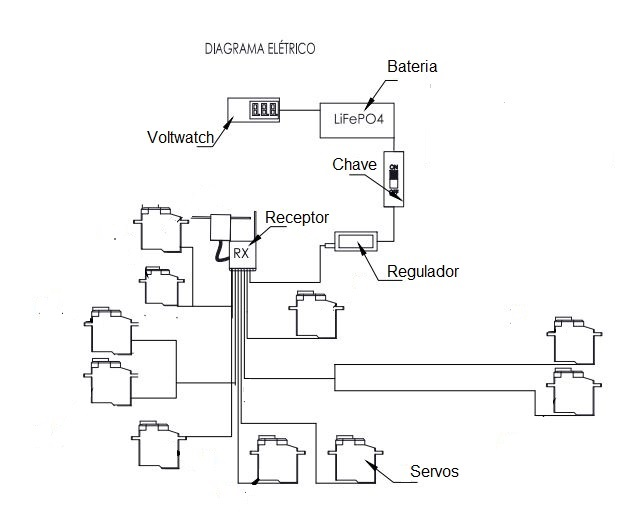
\includegraphics[width=0.6\textwidth]{./Imagens/Diagrama_eletrico}
    \fonte{Equipe}
    \label{fig:diagrama_eletrico}
\end{figure}

\chapter{Obtenção e validação de dados}\label{dados.cap}

Com o objetivo de validar os cálculos teóricos a equipe optou pela utilização de um
sistema de telemetria, que consiste em um circuito eletrônico embarcado que faz diversas
medições e envia para uma base no solo em tempo real, podendo monitorar diversas variáveis
que influenciam no desempenho do avião durante o voo.

Diante das necessidades da equipe e pensando em um sistema que fosse adaptável;
podendo ser utilizado em diversos protótipos; e de fácil manutenção, foi desenvolvido um
sistema de telemetria próprio, tanto em hardware, quanto em software, focando mais nos
objetivos do projeto.

\section{Componentes}

Foi escolhido o Microcontrolador ATMEGA328 (1) devido a facilidade de compra no
mercado nacional e ao bom custo/benefício quando comparados a outros MCU compatíveis,
tais como PIC18F4550/PIC18F255 da Microchip ou a série MSP430G2x da Texas Instruments.

Para transferir os dados de maneira remota, optou-se pelo módulo APC220 (2), um par
de sensores que comunicam-se através de radiofrequência, que pode ser alterada entre 418 e
455 MHz, e possui uma interface serial para leitura e envio de dados. A frequência de 418 MHz
foi escolhida por obter maior distância de comunicação nos campos de testes da equipe com
Baudrate de 9600 bps e alcance de 800 m, suficiente para comunicação e segurança da estação
de solo.

Com o objetivo de minimizar o risco de perda de dados por possíveis falhas no sinal, foi
utilizado um cartão de memória (3) embarcado, sendo possível analisar todo os dados do voo
posteriormente, sem nenhuma falha ou perda de informações.

O sensor GPS NEO-6M foi utilizado para traçar a rota do protótipo, fornecendo o
posicionamento geográfico (latitude/longitude), velocidade, data e hora, quantidade de satélites
captados, altitude, dentre outros dados não utilizados.

Os chips ADXL345 e L3G4200D fornecem valores da aceleração do deslocamento
vertical e rotacional, respectivamente, nos três eixos. Com esses dados são validados valores de
pitch e o roll durante o voo.

Para complementar, foi adicionado ao Hardware o Chip HMC5883L que é capaz de
medir o campo magnético da terra e indicar em qual sentido o nosso protótipo está deslocando.
Além de todos citados, com o Chip BMP085 é possível mensurar a temperatura e pressão
atmosférica, que, juntamente com o tubo de pitot, mede a velocidade relativa.

Para facilitar a construção do Hardware, foi utilizado um módulo (4) que une todos os
chips listados, de forma que foi possível realizar a comunicação individual com cada um,
através do protocolo I2C. Além disso, para aumentar a propriedade adaptativa do circuito, a
equipe utilizou barras de pino com sequência específica para adaptação ao hardware da maioria
dos sensores analógicos. Tal sequência consiste em um conjunto de 4 pinos para cada porta
analógica do MCU, tal que, por padrão, seguem a seguinte ordem: Ground–5V–SINAL–
Ground (5). Diante dessa configuração, podemos ligar de maneira simplória sensores que
possuem padrão distinto do normalmente utilizado em aeromodelismo (Ground –5V-SINAL),
tais como, 5V–SINAL– Ground.

É de extrema importância a medição de componentes elétricas como tensão e corrente
durante todo o voo. Para isso, foi utilizado o sensor ACS712 para a medição da corrente total
demandada por toda a aeronave e as correntes em cada servo separadamente. Para medir a
tensão, foi aplicado um simples circuito divisor de tensão, para adequar os valores da bateria
7utilizada aos valores do conversor analógico-digital do MCU.

\begin{figure}[h]
    \centering
    \caption{Circuito Parcial da Telemetria Utilizada}
    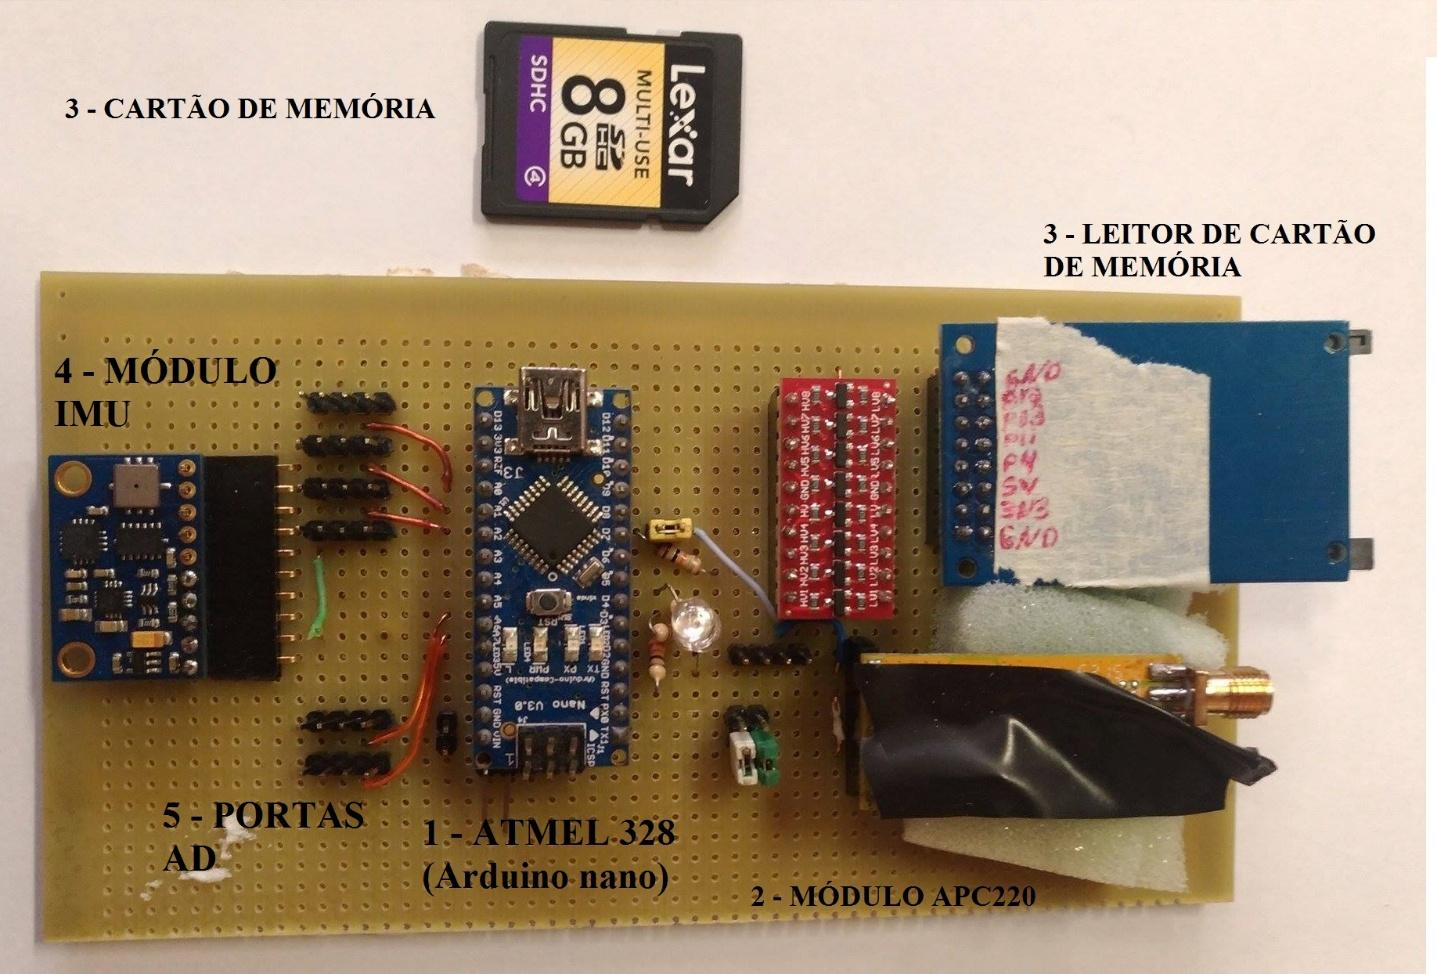
\includegraphics[width=0.8\textwidth]{./Imagens/Circuito_parcial_da_telemetria}
    \fonte{Equipe}
    \label{fig:telemetria}
\end{figure}

\chapter{Demandas}\label{demandas.cap}

De acordo com a telemetria empregada em nossos protótipos e testes estáticos nos
componentes e cálculos analíticos, foi possível mensurar as principais demandas elétricas da
aeronave. A seguir haverá o detalhamento da aquisição de dados das demandas de torque e
corrente do projeto.

\section{Determinação de demandas}

De acordo com a tabela de inputs, estão listados abaixo os torques requeridos de cada
servo.

\begin{table}[h]
\centering
\caption{Torques calculados para cada servo}
\label{tab:torque_requerido}
\begin{tabular}{|c|c|}
\hline
\multicolumn{1}{|l|}{\textbf{Dispositivo}} & \multicolumn{1}{l|}{\textbf{Torques Requeridos(Kgf*cm)}} \\ \hline
Servo1                                     & 0,89                                                     \\ \hline
Servo2                                     & 3,47                                                     \\ \hline
Servo3                                     & 3,56                                                     \\ \hline
Servo4                                     & 8,90                                                     \\ \hline
Servo5                                     & 3,90                                                     \\ \hline
Servo6                                     & 3,90                                                     \\ \hline
Servo7                                     & 1,02                                                     \\ \hline
Servo8                                     & 1,02                                                     \\ \hline
Servo9                                     & 4,10                                                     \\ \hline
Servo10                                    & 4,10                                                     \\ \hline
\end{tabular}
\end{table}

\section{Correntes}

Para determinar a curva característica de corrente em função do torque aplicado, para
cada servo, a equipe realizou o teste de carga com medição de corrente, dessa forma foi possível
analisar de forma mais ampla as configurações e variações de corrente nos servos. No teste, foi
variada a carga inserida no atuador sendo medida a corrente, através da telemetria.
Posteriormente, foi feito a utilização do método dos mínimos quadrados para a otimização
matemática dos resultados, obtendo dessa forma o modelo linear de Corrente x Torque [P.C.
Sen 1996], como demonstrado no Gráfico 1, que foi ilustrado n \autoref{fig:graf:corrente_torque}.

\begin{figure}[H]
    \centering
    \caption{Montagem corrente x torque}
    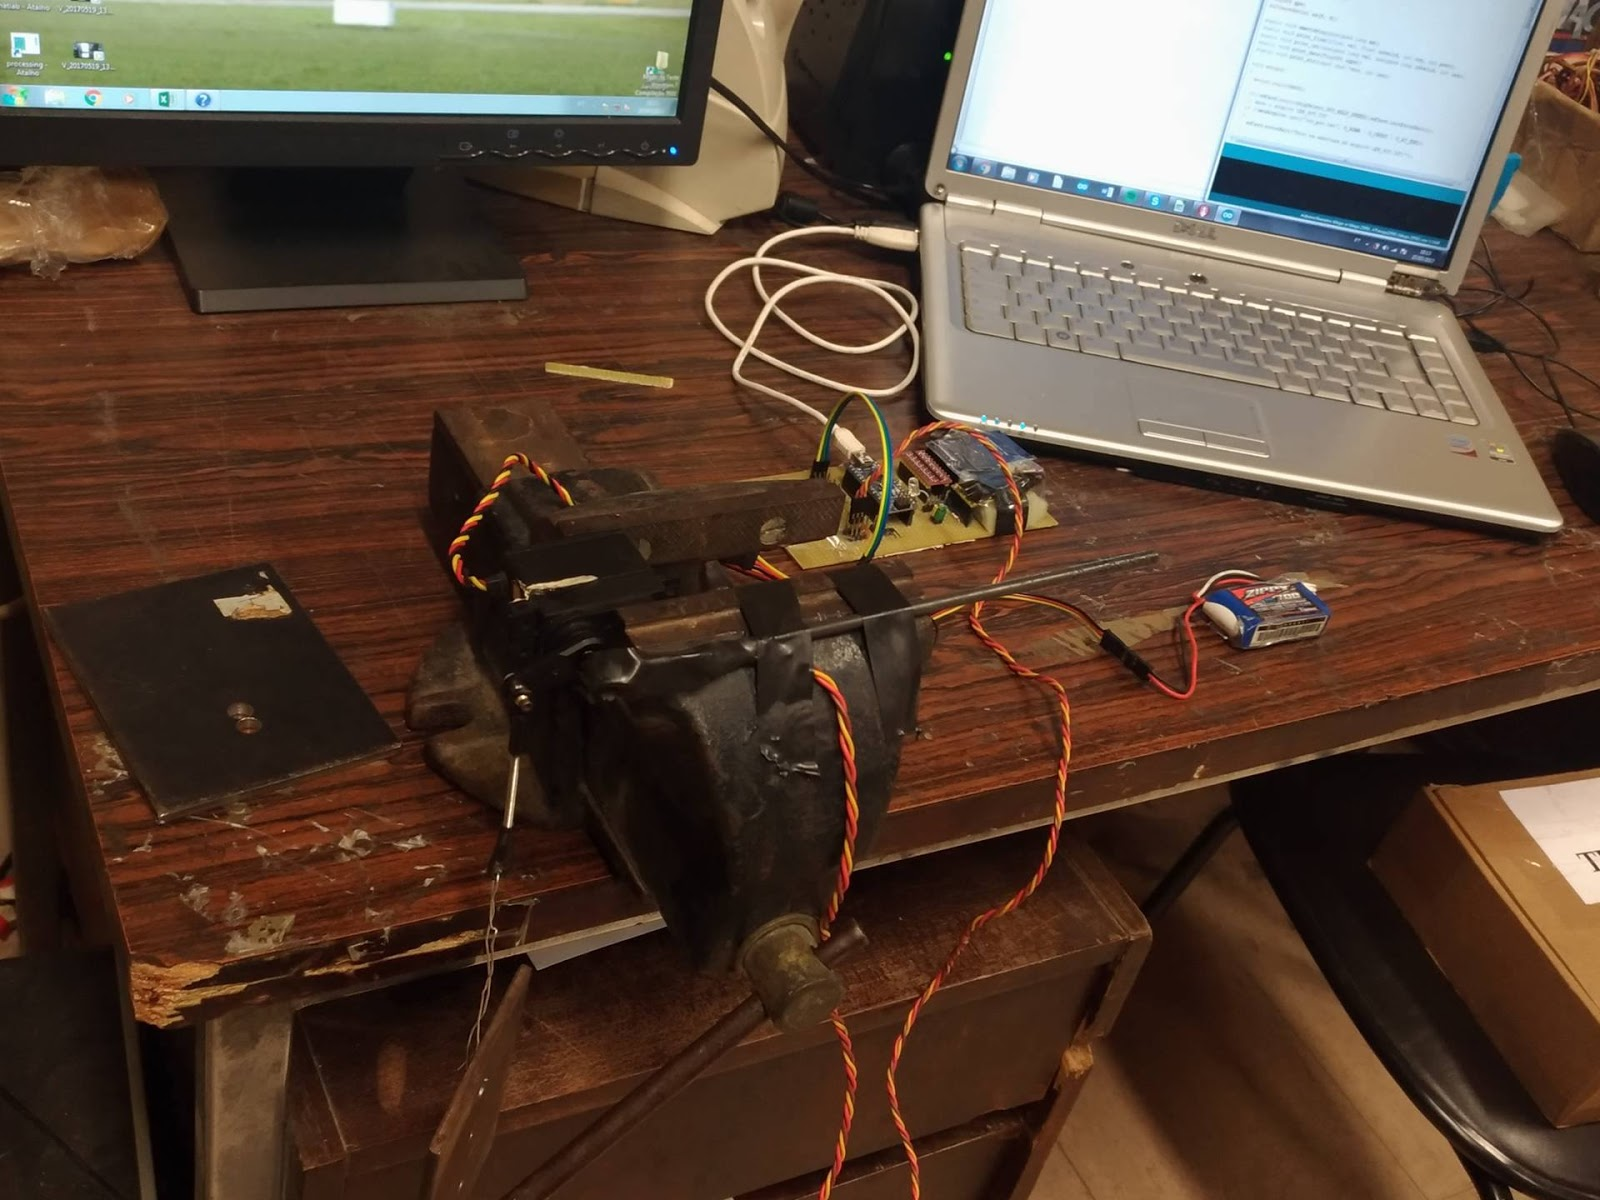
\includegraphics[width=0.8\textwidth]{./Imagens/Montagem}
    \fonte{Equipe}
    \label{fig:montagem}
\end{figure}

\begin{figure}[H]
    \centering
    \caption{Ilustração do gráfico Corrente(mA) x Torque (KGF.cm)}
    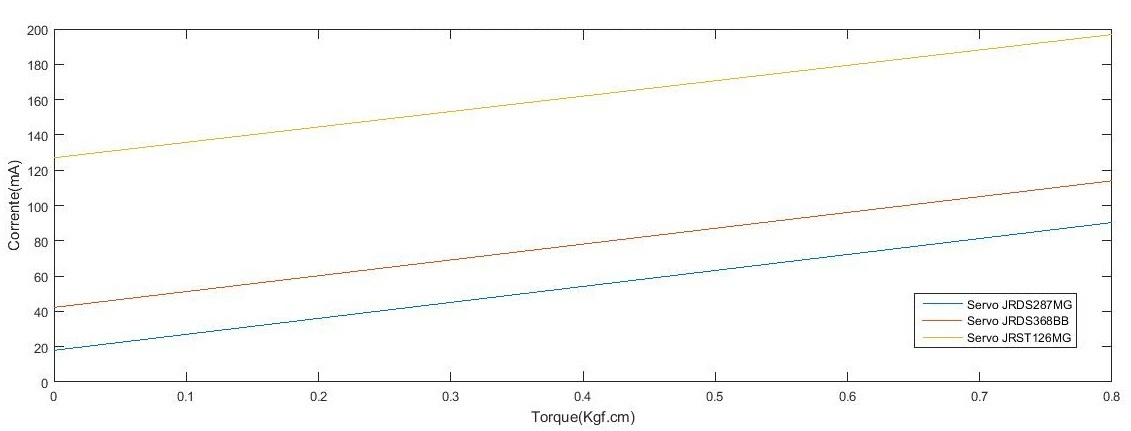
\includegraphics[width=0.8\textwidth]{./Imagens/Grafico_corrente_torque}
    \fonte{MATLAB®}
    \label{fig:graf:corrente_torque}
\end{figure}

Com o método dos mínimos quadrados utilizado no MATLAB®, foi possível notar que
o resultado do experimento é satisfatório, visto que os resultados das correntes para os torques
requeridos foram próximos de acordo com a telemetria empregada durante os voos da equipe,
com uma variação de 5\% para mais ou para menos.

\begin{table}[H]
\centering
\caption{Equações da corrente em função do torque}
\label{tab:equacoes}
\begin{tabular}{|c|c|}
\hline
\textbf{Modelo}    & \textbf{Corrente}       \\ \hline
\textit{JRDS287MG} & i = 90,481  T + 17,945 \\ \hline
\textit{JRDS368bb} & i = 89,66  T + 42,259  \\ \hline
\textit{JRST126MG} & i = 87,256  T + 127,05 \\ \hline
\end{tabular}
\end{table}

De acordo com as equações acima, foi possível prever a corrente para a carga requerida,
a \autoref{tab:corrente_maxima} demonstra os resultados obtidos.

\begin{table}[H]
\centering
\caption{Corrente demandada de acordo com a carga exigida}
\label{tab:corrente_maxima}
\begin{tabular}{|l|l|}
\hline
\textbf{Dispositivo} & \textbf{Corrente Máxima(mA)} \\ \hline
\textit{Servo1}      & 98,483                       \\ \hline
\textit{Servo2}      & 353,379                      \\ \hline
\textit{Servo3}      & 361,448                      \\ \hline
\textit{Servo4}      & 903,628                      \\ \hline
\textit{Servo5}      & 391,933                      \\ \hline
\textit{Servo6}      & 391,933                      \\ \hline
\textit{Servo7}      & 110,235                      \\ \hline
\textit{Servo8}      & 110,235                      \\ \hline
\textit{Servo9}      & 409,865                      \\ \hline
\textit{Servo10}     & 409,865                      \\ \hline
\end{tabular}
\end{table}

\chapter{Escolha dos Componentes}\label{escolha_componentes.cap}
\section{Bateria}

De acordo com diversos ensaios e testes feitos de forma dinâmica e estática, dentre as
possibilidades permitidas pelo regulamento, a equipe optou pela bateria LiFePO 4 de 500mAh
15C de 6.6Vda fabricante ProTek RC.

\begin{figure}[H]
    \centering
    \caption{Bateria ProTek 500mAh}
    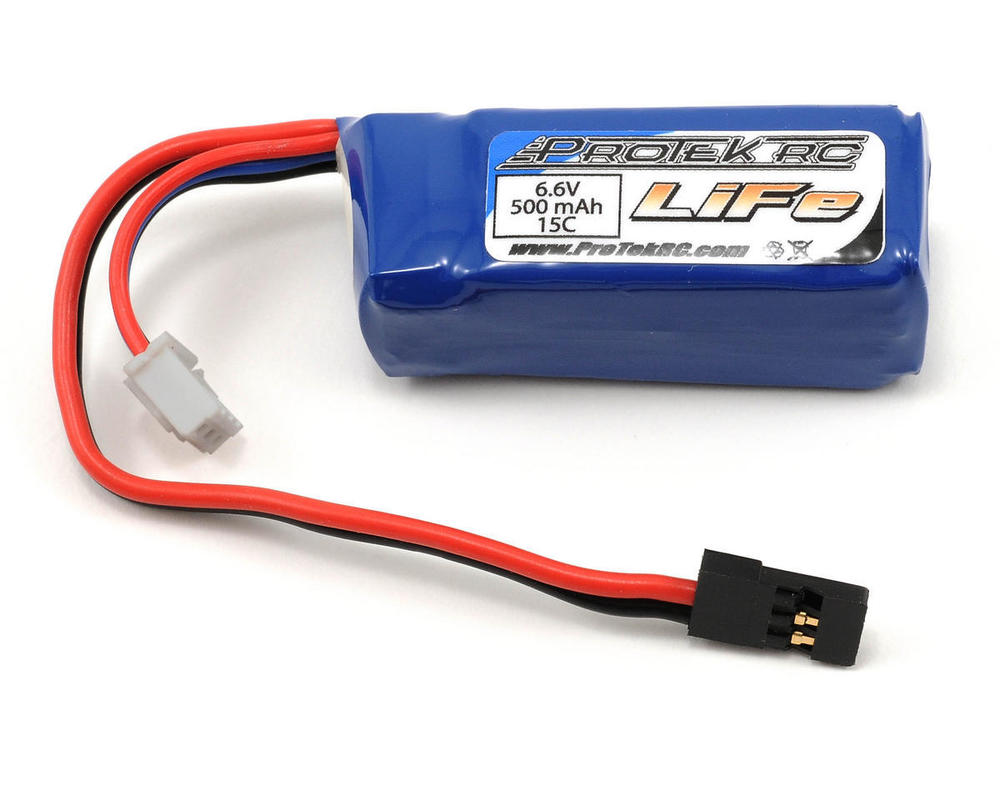
\includegraphics[width=0.8\textwidth]{./Imagens/bateria}
    \fonte{ebay}
    \label{fig:bateria}
\end{figure}

Para a escolha de tal bateria, foi realizado um teste de consumo via Extreme Power
Analyzer, wattímetro ilustrado na Figura 5, com intuito de confirmar o consumo de corrente
durante uma missão com um tempo de voo de 195,0 s, além do tempo na área de inspeção, que
durou aproximadamente 70 s. A carga total requerida foi de 390,23mAh, aumento
aproximado de 80\% quando comparado ao nosso protótipo anterior, justificado pela
inclusão de mais 4 servos (2 flaps e 2 freios), que demandam alta carga, principalmente
na hora do pouso e da decolagem. Aplicando FS obtivemos um consumo final adotado de
aproximadamente 448,76mAh. Comercialmente, o valor mais próximo e com o melhor custo
benefício, foi a bateria citada anteriormente, com carga total de 500mAh.

\begin{figure}[H]
    \centering
    \caption{Extreme Power Analyzer}
    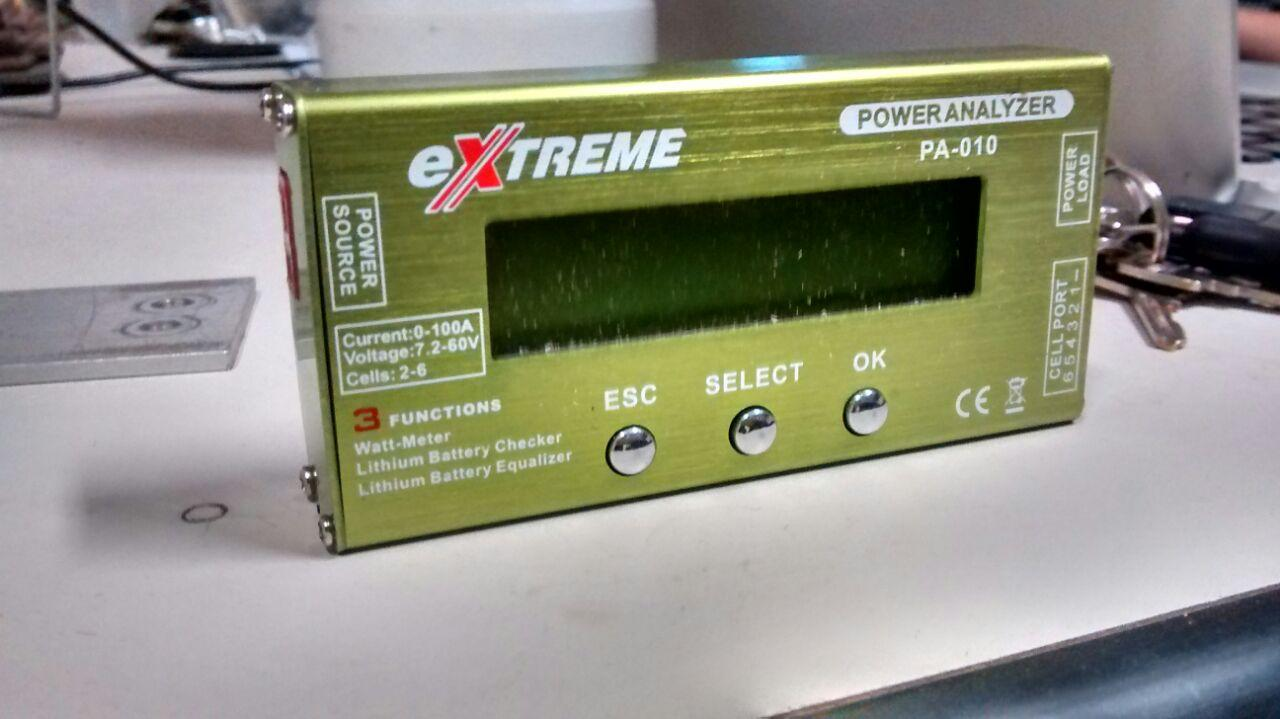
\includegraphics[width=0.8\textwidth]{./Imagens/extreme}
    \fonte{RCECHO}
    \label{fig:extreme}
\end{figure}

\section{Servos}

Para selecionar os servos, primordialmente, foi levado em consideração os cálculos
teóricos de torque máximo para cada superfície móvel da aeronave. Após saber o esforço que
cada servo será exposto, a equipe escolheu, dentre as marcas disponíveis no mercado, aquela
que possui uma melhor relação entre três fatores importantes, sendo eles o menor peso, a melhor
qualidade de construção e a que demonstrou melhor durabilidade por experiência da equipe.

A \autoref{tab: desc.servo} demonstra as especificações dos componentes escolhidos.

\begin{table}[H]
\centering
\caption{Descrição dos servos utilizados e torque do fabricante}
\label{tab: desc.servo}
\begin{tabular}{|c|c|c|c|c|}
\hline
\textbf{Dispositivo} & \textbf{Função}  & \textbf{Modelo} & \textbf{Massa(g)} & \textbf{TMF(N.m)} \\ \hline
\textit{Servo1}      & Acelerador       & JRDS287MG       & 13                & 0,113             \\ \hline
\textit{Servo2}      & Bequilha         & JRDS368BB       & 25                & 0,423             \\ \hline
\textit{Servo3}      & Leme             & JRDS368BB       & 25                & 0,423             \\ \hline
\textit{Servo4}      & Profundor        & JRST126MG       & 47                & 1,003             \\ \hline
\textit{Servo5}      & Aileron direito  & JRDS368BB       & 25                & 0,423             \\ \hline
\textit{Servo6}      & Aileron esquerdo & JRDS368BB       & 25                & 0,423             \\ \hline
\textit{Servo7}      & Freio direito    & JRDS287MG       & 13                & 0,113             \\ \hline
\textit{Servo 8}     & Freio esquerdo   & JRDS287MG       & 13                & 0,113             \\ \hline
\textit{Servo 9}     & Flap direito     & JRDS368BB       & 25                & 0,423             \\ \hline
\textit{Servo 10}    & Flap esquerdo    & JRDS368BB       & 25                & 0,423             \\ \hline
\end{tabular}
\end{table}

\section{Regulador de Tensão}

Sem a utilização do regulador de tensão, seria aplicado a tensão da bateria, que, em
servos comuns, é superior a sua tensão de funcionamento, o que causaria danos ao sistema
elétrico dos servos. Diante disso, para um sistema sem o regulador, seria necessário alterar todos
os servos para modelos que suporte tal tensão, conhecidos como servos High-voltage. O
principal ponto positivo de tal sistema é a economia de peso, devido a ausência de um UBEC,
porém, como os servos serão ligados diretamente na bateria, ao longo do voo a tensão da bateria
tende a diminuir, devido a demanda e descarga, diminuindo o torque máximo suportado pelo
servo, sendo necessário um superdimensionado a fim de garantir o torque necessário em tensões
mais baixas do que a nominal do servo.

Utilizando o regulador de tensão, opção escolhida pela equipe, acrescentamos peso ao
sistema elétrico, portanto, temos uma tensão fixa e igual à nominal do servo, garantindo um
torque máximo constante, proporcionando a segurança e o funcionamento correto de todo o
sistema elétrico durante o voo.

Considerando os valores fornecidos na \autoref{tab:corrente_maxima} Tabela 2, totalizou-se um valor de corrente máximo de 3541mA, que somado a corrente necessária para alimentar o receptor e o satélite, aproximadamente 500mA de acordo com o fabricante, resultaria em um total de 4041mA, que
após aplicação do FS, obtemos 4647,15mA . Diante desses dados, foi escolhido o UBEC
Turnigy 6V/8A, que se enquadra dentro de todos os parâmetros necessários de corrente e tensão
e possui chave geral (\autoref{fig:regulador}) de acordo com os requisitos impostos pelo regulamento da
competição, desligando o circuito referente ao receptor e aos servos.

\begin{figure}[H]
    \centering
    \caption{UBEC Turnigy 8A}
    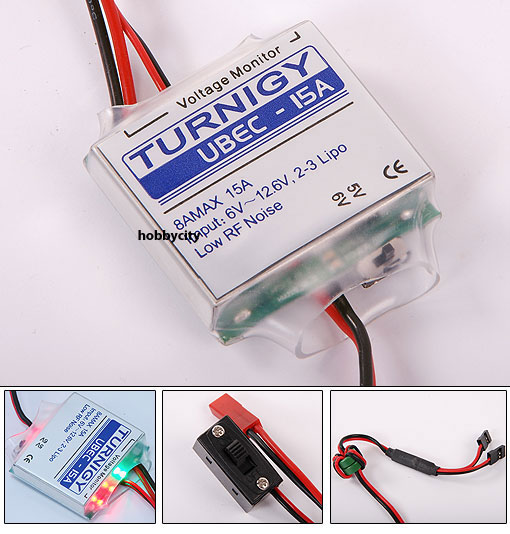
\includegraphics[width=0.8\textwidth]{./Imagens/regulador}
    \fonte{HobbyKing}
    \label{fig:regulador}
\end{figure}

\section{Receptor}

O receptor AR8000 DSMX® high-speed 8-channel receiver foi o escolhido por se
adequar melhor às demandas do projeto. Tal escolha foi feita a partir da análise da quantidade
de servomotores presentes na aeronave, das especificações de distância em que o mesmo atua
e facilidade de compra do mesmo. O receptor escolhido tem dois canais a menos que a
quantidade de servos da aeronave, para correção desse fato foi utilizado uma extensão em Y
para os servos do aileron e do freio, de forma que fosse possível o comando para todos os
servomotores e mantendo um equilibrio de massa na asa, já que os servos do aileron são
posicionados de maneira simétrica devido ao sinal enviado a eles.

Algumas características do AR8000 DSMX® podem ser ressaltadas, como sua
blindagem eletromagnética, que é produzida por sua estrutura de fibra de carbono, e evita a
livre passagem de ondas eletromagnéticas pelo receptor. Outra característica marcante é a alta
14velocidade de resposta do receptor, sendo esse um diferencial para os comandos das superfícies
móveis.

\chapter{Projeto da Fiação}\label{fio.cap}

A fim de obter a menor perda de potência possível, respeitando as dimensões do projeto,
e minimizando o gasto excessivo de material, foram realizas medidas dos comprimentos para
cada fiação do seu respectivo servo até seu canal equivalente no receptor. Dessa forma a equipe
pôde confeccionar cabos de tamanhos mais apropriados, de acordo com a \autoref{tab:comp_fio}.

\begin{table}[H]
\centering
\caption{Comprimento da fiação para cada conexão}
\label{tab:comp_fio}
\begin{tabular}{|c|c|}
\hline
\textbf{Conexões}         & \textbf{Comprimento (m)} \\ \hline
\textit{Leme}             & 0,625                    \\ \hline
\textit{Aileron Esquerdo} & 1,07                     \\ \hline
\textit{Aileron Direito}  & 1,07                     \\ \hline
\textit{Profundor}        & 0,83                     \\ \hline
\textit{Flap Esquerdo}    & 1,74                     \\ \hline
\textit{Flap Direito}     & 1,74                     \\ \hline
\textit{Bequilha}         & 0,93                     \\ \hline
\textit{Motor}            & 0,94                     \\ \hline
\textit{Freio Esquerdo}   & 0,13                     \\ \hline
\textit{Freio Direito}    & 0,13                     \\ \hline
\end{tabular}
\end{table}

\section{Tipo de Cabeamento}

A escolha do tipo de cabeamento se restringiu aos cabos AWG 24 e AWG 26 (\autoref{tab:esp_cabos}), visto que os mesmos são mais fáceis de serem comprados, com maior confiabilidade. A
Tabela 5 demonstra as principais características dos tipos de AWG, o que será necessário para
efetuar os cálculos posteriores.

\begin{table}[H]
\centering
\caption{Especificações básicas dos cabos}
\label{tab:esp_cabos}
\begin{tabular}{|c|c|c|c|}
\hline
\textbf{Bitola AWG} & \textbf{Diâmetro (mm)} & \textbf{Ohms por km (T = $20\,^{\circ}\mathrm{C}$)} & \textbf{Corrente máxima} \\ \hline
\textit{23}         & 0.57404                & 20.36                           & 4.7                      \\ \hline
\textit{24}         & 0.51054                & 25.67                           & 3.5                      \\ \hline
\textit{25}         & 0.45466                & 32.37                           & 2.7                      \\ \hline
\textit{26}         & 0.40386                & 40.81                           & 2.2                      \\ \hline
\textit{27}         & 0.36068                & 51.27                           & 1.7                      \\ \hline
\end{tabular}
\end{table}

A partir dos dados acima e do comprimento dos condutores de cada conexão, pôde-se
calcular a resistência intrínseca de cada um deles a uma temperatura de 20oC para ambas as
bitolas. Por fim, a \autoref{tab:res_cabos} segue com os resultados dos cálculos de resistência para os cabos 15AGW 24 e AGW 26, respectivamente.

\begin{table}[H]
\centering
\caption{Resistências mensuradas dos cabos AWG 24 e 26}
\label{tab:res_cabos}
\begin{tabular}{|c|c|c|}
\hline
\textbf{Conexões}  & \textbf{Resistência AWG 24} & \textbf{Resistência AWG 26} \\ \hline
\textit{Leme}      & 0,0526235                   & 0,0836605                   \\ \hline
\textit{Ailerons}  & 2 x 0,090091432             & 2 x 0,143226776             \\ \hline
\textit{Profundor} & 0,069884008                 & 0,111101144                 \\ \hline
\textit{Flaps}     & 2 x 0,146503824             & 2 x 0,232910832             \\ \hline
\textit{Freios}    & 2 x 0,010945688             & 2 x 0,017401384             \\ \hline
\textit{Motor}     & 0,079145744                 & 0,125825392                 \\ \hline
\textit{Bequilha}  & 0,078303768                 & 0,124486824                 \\ \hline
\end{tabular}
\end{table}

Com o objetivo de evitar qualquer tipo de falha técnica no circuito elétrico, garantindo
maior segurança em voo, de acordo com as tabelas acima a escolha mais sensata foi o cabo
AWG 24 por apresentar uma menor resistência e consequentemente uma menor dissipação de
potência. Apesar do AWG 26 apresentar massa relativamente menor, não é relavante quando
comparado ao outro cabo analisado.

\chapter{Lista de Outputs}\label{output.cap}

\begin{table}[H]
\centering
\caption{Lista de Outputs}
\label{tab:outputs}
\begin{tabular}{|c|c|c|c|}
\hline
\multicolumn{4}{|c|}{\textbf{OUTPUTS}}                                                                                     \\ \hline
\textit{\textbf{Variáveis}}           & \textit{\textbf{Valor}} & \textit{\textbf{Unidades}} & \textit{\textbf{Relatório}} \\ \hline
\textit{Velocidade de decolagem}      & 11,8                    & m/s                        & Desempenho                  \\ \hline
\textit{Tempo máximo de voo}          & 195                     & Segundos                   & Desempenho                  \\ \hline
\textit{Torque do servo do profundor} & 1,003                   & N.m                        & Estabilidade                \\ \hline
\end{tabular}
\end{table} 		% Aerodinamica
% ---
% Conclusão
% ---
\chapter{Conclusão}
% ---
Se é que terá um capítulo de conclusão..
% ----------------------------------------------------------
% ELEMENTOS PÓS-TEXTUAIS
% ----------------------------------------------------------
\postextual

% ----------------------------------------------------------
% Referências bibliográficas
% ----------------------------------------------------------
\bibliography{aero}

\end{document}
